\documentclass[french, a4paper, 12pt]{article}

%French setting up
\usepackage[utf8]{inputenc}
\usepackage[T1]{fontenc}
\usepackage{babel}

\setlength{\parindent}{0cm}
\usepackage{amsmath}
\usepackage{siunitx} %physics units
\usepackage{graphicx} % Images
\graphicspath{ {./images/} }
\usepackage{fancyhdr}

%Border
\usepackage[left=1in, right=1in, top=1in, bottom=1in]{geometry}
 
\pagestyle{fancy}
\fancyhf{}
\rhead{ImmortalPharaoh7}
\lhead{Notes de Révision Physique NS}
\cfoot{\thepage}

\author{ImmortalPharaoh7}
\title{Notes de Révision Physique NS}
\date{Mai 2020}

\usepackage{hyperref} %Last package
\urlstyle{same}
\begin{document}
\begin{titlepage}
\maketitle
\begin{abstract}
Les notes de révision pour la physique niveau supérieur du BI, pour le curriculum qui commence dès 2016. Attention, ces notes ne sont pas à être utilisées indépendamment; ils servent comme des astuces ou bien les définitions qui peuvent être oubliées.

Si vous avez des informations à ajouter ou bien des corrections, veuillez envoyer un email à pharaoh.immortal7@gmail.com ou messager ImmortalPharaoh7\#7811 sur Discord.
\end{abstract}
\end{titlepage}

\pagenumbering{roman}
\tableofcontents
\pagebreak

\pagenumbering{arabic}
\section{Mesures et Incertitudes}
\subsection{Unités de Système Internationale}
\textbf{Unités de Système Internationale:}
\begin{itemize}
\item Masse: en kilogramme (kg)
\item Longueur: en mètre (m)
\item Temps: en seconde (s)
\item Courant électrique: en ampère (A)
\item Quantité de matière: en mol (mol)
\item Température: en Kelvin (K)
\item Luminosité: en candela (cd)
\end{itemize}
Pour les autres unités:
\begin{figure}[h]
\centering
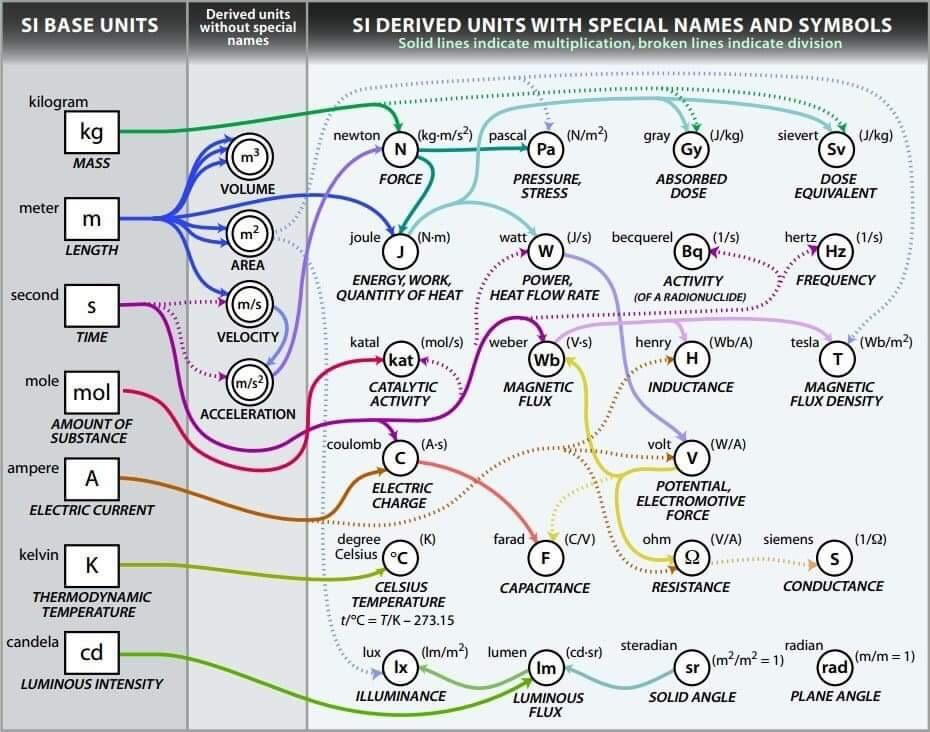
\includegraphics[scale=0.4]{units_derivation}
\end{figure}

\subsection{Incertitudes et Erreurs}
Attention: faire des opérations avec des nombres constantes ne changent pas l'incertitude.\\
Calculer l'erreur aléatoire: $\frac{a_{max}-a_{min}}{2}$.
\pagebreak

\section{Mécanique}
\subsection{Mouvement}
\textbf{Définitions:}
\begin{itemize}
\item Déplacement: Distance parcouru dans une direction (en \si{\metre}).
\item Vitesse: Taux de variation de déplacement (en \si{\metre\per\second}).
\item Accélération: Taux de variation de vitesse (en \si{\metre\per\second\squared}).
\end{itemize}
La dérivée du déplacement est la vitesse. La dérivée de la vitesse est l'accélération.\\
Attention: Quand on traite un problème de 2 dimensions, il faut toujours séparer les dimensions.

\subsection{Forces}
\textbf{Définitions:}
\begin{itemize}
\item Force: La masse fois l'accélération (en \si{\newton} ou \si{\kilogram\metre\per\second\squared}).
\item Frottement: La force qui est appliquée entre deux objets on contact.
\item Première loi de Newton: Si un objet ne subit aucune force, il est soit au repos ou en mouvement rectiligne uniforme.
\item Deuxième loi de Newton: La somme des forces réagissant sur un objet $F=ma$.
\item Troisième loi de Newton: Si un objet A exerce une force sur un objet B, alors objet B exerce une force sur A de même grandeur et de sens opposé $F_{BA}=-F_{AB}$.
\end{itemize}
Dans la situation d'un plan incliné, la force résultante est $=mg\sin \theta$ et la réaction normale $=mg\cos \theta$.\\
Attention: Le coefficient de frottement statique dans le cas du plan incliné $\mu _s =\tan\theta_{max}$.

\subsection{Travail, Énergie et Puissance}
\textbf{Définitions:}
\begin{itemize}
\item Travail: Force net fois le déplacement (en \si{\joule} ou \si{\newton\metre}).
\item Énergie: La mesure du travail effectué (en \si{\joule} ou \si{\newton\metre}).
\item Énergie cinétique: L'énergie dû à la vitesse $E_c=\frac{1}{2}mv^2$.
\item Énergie potentielle: L'énergie dû à la position $E_p=mgh$, et dans le cas d'un ressort $E_p=\frac{1}{2}k\Delta x^2$.
\item Puissance: Taux de transfert d'énergie (énergie/temps) (en \si{\watt} ou \si{\joule\per\second}).
\item Rendement: Le pourcentage d'énergie / puissance utile.
\end{itemize}
Attention: Si un objet se déplace à une vitesse constante contre une force de frottement, alors la puissance $P=Fv$.

\subsection{Quantité de Mouvement et Impulsion}
\textbf{Définitions:}
\begin{itemize}
\item Quantité de mouvement: Masse fois la vitesse (en \si{\kilogram\metre\per\second} ou \si{\newton\second}).
\item Impulsion: $\Delta p$, utilisée dans la deuxième loi de Newton.
\item Choc élastique: Choque dans lequel il n'y aucune perte d'énergie.
\item Choc inélastique: Choque dans lequel il y a une perte d'énergie. Un choc complètement inélastique résulte que les objets restent collés.
\end{itemize}
Attention: Quand la masse n'est pas constante, la deuxième loi de Newton devient $F=\dfrac{\Delta p}{\Delta t}$.\\
Attention: L'impulsion est nulle seulement si la force résultante dans le système est nulle (système est isolé).

\section{Physique Thermique}
\subsection{Concepts de Thermique}
\textbf{Définitions:}
\begin{itemize}
\item Chaleur: Énergie dû à l'énergie cinétique dans ses particules.
\item Capacité thermique d'une matière: L'énergie nécessaire pour augmenter la température de la matière de 1 K.
\item Chaleur latente: Énergie nécessaire pour que la matière change de phase. Cette énergie est utilisée pour augmenter l'énergie potentielle entre les molécules.
\end{itemize}

\subsection{Modélisation d'un Gaz}
\textbf{Définitions:}
\begin{itemize}
\item Loi des gazes parfaits: $pV=nRT$. Très important à savoir.
\item Gaz parfait: Un gaz qui respecte la loi des gazes parfait. En plus, il n'y a pas des forces intermoléculaires et les collisions entre les molécules sont complètement élastiques.
\item Pression: La force par unité de surface (en \si{\pascal}).
\end{itemize}
Attention: Pour résoudre un problème des gazes parfaits, il faut mettre tout les variables dans un côté et les constantes dans l'autre et donc $\text{Variable}_1=\text{Variable}_2$.
\pagebreak

\section{Ondes}
\subsection{Oscillations}
\textbf{Définitions:}
\begin{itemize}
\item Période $T$: Durée d'une oscillation complète (en \si{\second}).
\item Fréquence $f$: Nombre de période par seconde (en \si{\hertz}).
\item Amplitude $A$: Déplacement maximal.
\item Longueur d'onde $\lambda$: Distance entre 2 points en phases.
\item Mouvement Harmonique Simple: Mouvement ondulatoire dans lequel l'accélération est proportionnelle à l'opposé du déplacement ($a\propto -x$).
\item Différence de Phase: Différence en $2\pi$ entre les phases des ondes, avec une différence de $\pi$ qui est considérée \og Opposition de phase \fg{}.
\end{itemize}
Attention: Dans un MHS, la période ne dépend pas de l'amplitude.\\
Dans un MHS: $E_T \propto m$, $E_T \propto A^2$ et $E_T \propto f^2$.

\subsection{Ondes Progressives}
\textbf{Définition:}
\begin{itemize}
\item Onde transversale: Onde dans laquelle le mouvement des particules est perpendiculaire à la direction de l'onde.
\item Onde longitudinale: Onde dans laquelle le mouvement des particules est parallèle à la direction de l'onde, il y a des compressions et des raréfaction (dilatations).
\end{itemize}
Attention: Dans un changement de milieu, la fréquence ne change pas; seulement la vitesse et la longueur d'onde.

\subsection{Caractéristiques des ondes}
\textbf{Définitions:}
\begin{itemize}
\item Intensité $I$: La puissance par unité de surface reçue (en \si{\watt\per\meter\squared}) avec $I \propto x^{-2}$ et $I \propto A^2$.
\item Superposition: Quand il y a une interférence avec plusieurs ondes, il peut y avoir soit une interférence soit constructive ou destructive, selon la différence de phase.
\item Ondes cohérentes: Les ondes qui ont un déphasage constant et ont la même fréquence, c'est la contrainte pour avoir des interférences constructives ou destructives.
\item Polarisation: Quand l'onde électromagnétique a une seule direction de propagation; une lumière non-polarisée est une lumière qui se propage dans toute les directions. Quand une lumière non-polarisée passe dans un polariseur, elle perd la moitié de son intensité.
\item Loi de Brewster: Une lumière réfléchie est totalement polarisée si et seulement si $\theta _{refl}+\theta_{refr}=90^\circ$ et donc $n_2=\tan \theta _i$.
\item Loi de Malus: Quand une lumière polarisée passe par un analyseur, l'amplitude finale sera $A=A_0 \cos \theta$ et par la suite $I=I_0 \cos ^2 \theta$.
\end{itemize}
Attention: Pour résoudre une question qui te donne l'intensité avec sa distance et te demande de chercher l'intensité avec l'autre distance, il suffit de faire 
\[
\frac{I_1}{I_2}=\frac{x_1^{-2}}{x_2^{-2}}=\frac{x_2^2}{x_1^2}
\]
même principe avec l'amplitude mais la manipulation sera différente.

\subsection{Comportements des Ondes}
\textbf{Définitions:}
\begin{itemize}
\item Première loi de Descartes: L'angle incident est égale à l'angle réfléchi par rapport à la normale.
\item Angle critique: L'angle avec lequel il n'y pas de réfraction, $\sin \theta _2=1 \implies n_1 \sin _1=n_2$.
\item Diffraction: Quand la lumière s'étale après avoir passé par une ouverture ou autour d'un obstacle. La diffraction devient importante quand la longueur d'onde est comparable à la largeur de l'ouverture.
\item Différence de Chemin: La différence de phase entre les ondes qui détermine si l'interférence sera constructive ou destructive.
\item Principe de Huygens: Chaque point sur un front d'onde émet une ondelette sphérique de mêmes vitesse et longueur d'onde que l'onde originale.
\end{itemize}

\subsection{Ondes stationnaires}
\textbf{Définitions:}
\begin{itemize}
\item Onde stationnaire: Une onde dans laquelle il n'y a pas de transfert d'énergie. Les points qui ont un déplacement nul sont des nœuds et les points qui ont une amplitude maximum sont des ventres. C'est le résultat de la superposition et de la réflexion des ondes.
\item Première harmonique: Plus basse fréquence dans un système d'onde stationnaire.
\end{itemize}
Attention: Pour un système fermé-fermé et ouvert-ouvert, $\lambda _0= 2l$ et $f_n=nf_0$. Mais pour fermé-ouvert $\lambda _0= \frac{4l}{3}$ et $f_n=(2n-1)f_0$.
\pagebreak

\section{Électricité et Magnétisme}
\subsection{Champs Électriques}
\textbf{Définitions:}
\begin{itemize}
\item Coulomb: Unité de la charge, courant fois le temps (en \si{\coulomb} ou \si{\ampere\second}).
\item Champ électrique positif: Champ créé par une charge positive. Il est un champ sortant.
\item Champ électrique négatif: Champ créé par une charge négative. Il est un champ entrant.
\item Loi de Coulomb: La force entre deux charge est $\propto \dfrac{q_1q_2}{r^2}$.
\item Conducteur: Une matière est considérée comme conducteur si un courant peut passer. Ceci est dû aux électrons libres.
\item Potentiel d'énergie électrique: Énergie d'une charge dû à sa position dans un champ électrique en (\si{\joule}). Comme un objet dans un champs gravitationnel.
\item Différence de potentiel électrique: Différence d'énergie entre deux points dans un champ électrique, par unité de charge (en \si{\volt} ou \si{\joule\per\coulomb}).
\item Courant: Le mouvement des charges dans un circuit. Le circuit doit être fermé pour maintenir un courant. C'est également le taux mouvement de la charge (en \si{\ampere}).
\end{itemize}
Attention: Il y a toujours une conservation de la charge. Une charge positive va avec la direction du courant tandis qu'une charge négative va contre la direction du courant.

\subsection{Effet Thermique des Courants Électriques}
\textbf{Définitions:}
\begin{itemize}
\item Résistance: Le rapport entre la tension et l'intensité du courant. Plus la résistance est grande, plus on aura besoin de différence de potentiel pour que le courant passe (en \si{\ohm} ou \si{\volt\per\ampere}).
\item Loi d'Ohm: Un appareil qui respecte la loi d'Ohm est un appareil qui respecte cette relation: $V \propto I$; la résistance est constante.
\item Puissance: En électricité, la puissance est également la tension fois l'intensité.
\item Première loi de Kirchoff: Dans une jonction, $\sum i_{in} = \sum i_{out}$.
\item Deuxième loi de Kirchoff: Dans une boucle, $\sum V=0$.
\item Potentiomètre: Appareil à 3 bornes qui permet de varier la résistance pour des raisons expérimentales. Retenir le montage ci-dessous par cœur.
\end{itemize}
Attention: Avec la deuxième loi de Kirchoff, il faut choisir une direction (avec les aiguilles de la montre ou pas), ensuite additionner ou soustraire les tensions. Si la direction va du négatif vers le positif d'une pile alors on additionne la tension, sinon on soustrait. Si la direction va avec les résistances on soustrait sinon on additionne.\\
Attention: Les résistance s'additionnent en série $R_{total}=R_1+R_2+\cdots$. En dérivation $1/R_{total}=1/R_1+1/R_2+\cdots$.
\begin{figure}[h]
\centering
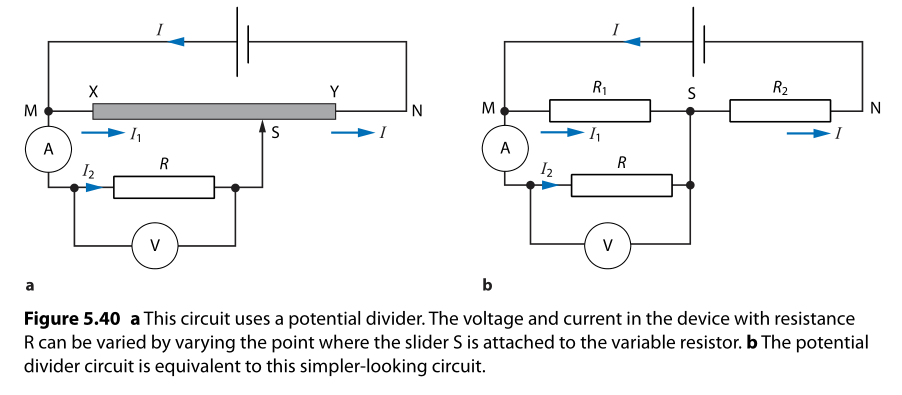
\includegraphics[scale=0.6]{potential_divider}
\end{figure}

\pagebreak

\section{Mouvement Circulaire et Gravitation}
\subsection{Mouvement Circulaire}
\textbf{Définitions:}
\begin{itemize}
\item Mouvement circulaire uniforme: Mouvement dans lequel la grandeur de la vitesse est constante mais il y a une force centripète qui agit sur l'objet en mouvement.
\item Force centripète: Force dirigée vers le centre qui est toujours perpendiculaire à la vitesse.
\item Vitesse angulaire: Vitesse de rotation (en \si{\radian\per\second})
\end{itemize}
Attention: La force résultante dans un mouvement circulaire uniforme c'est elle qui $=\dfrac{mv^2}{r}$.

\subsection{Loi de Gravitation de Newton}
\textbf{Définitions:}
\begin{itemize}
\item Champ gravitationnel: Champ qui est dû à la masse de l'objet. La force créée par le champ est toujours attractive.
\item Loi de gravitation de Newton: Chaque masse crée un champ gravitationnel autour d'elle et attire toutes les autres masses.
\end{itemize}
Attention: Dans les situations où il y 2 planètes et c'est demandé de savoir la force résultante ou bien l'accélération, il suffit de faire une addition vectorielle de chaque force. Donc c'est essentiel de savoir l'angle qui est entre ces deux forces.
\pagebreak

\section{Physique Atomique et Nucléaire}
\pagebreak

\section{Production d'Énergie}
\pagebreak

\section{Phénomènes Ondulatoire}
\subsection{Mouvement Harmonique Simple}
\textbf{Définitions:}
\begin{itemize}
\item Mouvement Harmonique Simple: Mouvement ondulatoire dans lequel l'accélération est proportionnelle à l'opposé du déplacement ($a\propto -x$).
\end{itemize}
Attention: Dans les formules du déplacement et de la vitesse du formulaire, il faut utiliser les formules qui sont à gauches quand le mouvement commence à l'équilibre et les formules qui sont à droites quand le mouvement commence du maximum.\\
L'énergie totale est conservé durant le mouvement tant qu'il n'y a pas d'amortissements.\\
Dans un MHS, la période ne dépend pas de l'amplitude.\\
Dans un MHS: $E_T \propto m$, $E_T \propto A^2$ et $E_T \propto f^2$.

\subsection{Diffraction par une seule fente}
\textbf{Définitions:}
\begin{itemize}
\item Diffraction: Quand la lumière s'étale après avoir passé par une ouverture ou autour d'un obstacle. La diffraction devient importante quand la longueur d'onde est comparable à la largeur de l'ouverture.
\end{itemize}
Angle entre $n$ minimum $\theta _n = 2n \lambda/b$ (Check this info).\\
Diffraction de la lumière blanche: Les couleurs avec la plus petite longueur d'onde (violet) sont plus proches du centre maximal, car l'angle de premier minimum diminue avec la longueur d'onde.\\
Attention: L'intensité du deuxième maximum est $I_0/20$, troisième est de $I_0/50$ et quatrième de $I_0/100$.

\subsection{Interférence}
\textbf{Définitions:}
\begin{itemize}
\item Réseau de diffraction: Un objet qui contient beaucoup de fentes avec la relation $n\lambda =d\sin \theta$ avec $n$ l'ordre de diffraction et $d$ la distance entre les fentes.
\item Interférence avec des lames minces: C'est l'interférence à cause d'une goutte ou une lame mince. L'interférence peut être constructive ou destructive selon l'indice de réfraction qui cause que les ondes reflètent soit en phase soit en opposition de phase.
\end{itemize}
En augmentant le nombre de fentes, la distance entre les franges (le $s$) reste constante mais les maximums sont plus prononcés et l'intensité varie comme ceci, pour l'intensité de maximum central
\[
I_N=N^2I_1
\]
pour $N$ le nombre de fentes.\\
Attention: Si $n_1 < n_2$ alors l'onde réfléchi sera en opposition de phase, sinon elle est en phase. L'onde transmise est toujours en phase.

\subsection{Résolution}
\textbf{Définitions:}
\begin{itemize}
\item Critère de Rayleigh: 2 sources sont justes résolues résolues si et seulement si le premier minimum de figure de diffraction de l'une des sources correspond au maximum central de la figure de diffraction de l'autre source. Selon l'angle, $\theta = \lambda /b$ pour une ouverture carré et $\theta = 1.22\lambda/b$ pour une ouverture circulaire (c'est l'angle minimum).
\end{itemize}
Question typique: donne la distance $d$ entre 2 sources et il faut trouver la distance minimum $D$. Il faut faire
\[
\frac{(1.22)\lambda}{b}=\frac{d}{D}
\]

\subsection{Effet Doppler}
\textbf{Définitions:}
\begin{itemize}
\item Effet Doppler: Le changement dans la fréquence reçue à cause de la vitesse relative entre la source et l'observateur.
\end{itemize}
Attention: Pour savoir s'il faut utiliser + ou -- dans la formule, il faut voire s'ils s'éloignent ou s'approchent. Dans le premier cas la fréquence augmente et dans l'autre elle diminue.
\pagebreak

\section{Champs}
\pagebreak

\section{Induction Électromagnétique}
\pagebreak

\section{Physique Quantique}
\pagebreak

\section{Astrophysique}
\end{document}